\documentclass[11pt]{article}
\usepackage{geometry,marginnote} % Pour passer au format A4
\geometry{hmargin=1cm, vmargin=1cm} % 

% Page et encodage
\usepackage[T1]{fontenc} % Use 8-bit encoding that has 256 glyphs
\usepackage[english,french]{babel} % Français et anglais
\usepackage[utf8]{inputenc} 

\usepackage{lmodern,numprint}
\setlength\parindent{0pt}

% Graphiques
\usepackage{graphicx,float,grffile,units}
\usepackage{tikz,pst-eucl,pst-plot,pstricks,pst-node,pstricks-add,pst-fun} 

% Maths et divers
\usepackage{amsmath,amsfonts,amssymb,amsthm,verbatim}
\usepackage{multicol,enumitem,url,eurosym,gensymb,tabularx}

\DeclareUnicodeCharacter{20AC}{\euro}



% Sections
\usepackage{sectsty} % Allows customizing section commands
\allsectionsfont{\centering \normalfont\scshape}

% Tête et pied de page
\usepackage{fancyhdr} \pagestyle{fancyplain} \fancyhead{} \fancyfoot{}

\renewcommand{\headrulewidth}{0pt} % Remove header underlines
\renewcommand{\footrulewidth}{0pt} % Remove footer underlines

\newcommand{\horrule}[1]{\rule{\linewidth}{#1}} % Create horizontal rule command with 1 argument of height

\newcommand{\Pointilles}[1][3]{%
  \multido{}{#1}{\makebox[\linewidth]{\dotfill}\\[\parskip]
}}

\newtheorem{Definition}{Définition}

\usepackage{siunitx}
\sisetup{
    detect-all,
    output-decimal-marker={,},
    group-minimum-digits = 3,
    group-separator={~},
    number-unit-separator={~},
    inter-unit-product={~}
}

\setlength{\columnseprule}{1pt}

\begin{document}

\textbf{Nom, Prénom :} \hspace{8cm} \textbf{Classe :} \hspace{3cm} \textbf{Date :}\\

\begin{center}
  \textit{Un tableau ne vit que par celui qui le regarde.}  - \textbf{Pablo Picasso}
\end{center}

\subsection*{ex1 : Restituer les formules de cours.}

\begin{multicols}{2}
\begin{itemize}
  \item Carré - Périmètre :\dotfill 
  \item Rectangle - Périmètre : \dotfill 
  \item Cercle - Périmètre : \dotfill
  \item Carré - Aire : \dotfill 
  \item Rectangle - Aire : \dotfill 
  \item Cercle - Aire : \dotfill
\end{itemize}
\end{multicols}

\subsection*{ex2 : Figures Compposées}
Il faut calculer les aires et les périmètres des figures suvantes. 

\begin{minipage}[t]{0.3\textwidth}
  \begin{figure}[H]
    \centering
    \includegraphics[width=0.7\linewidth]{5x5-aires-et-perimetres/ex1.pdf}
  \end{figure}

  \begin{figure}[H]
    \centering
    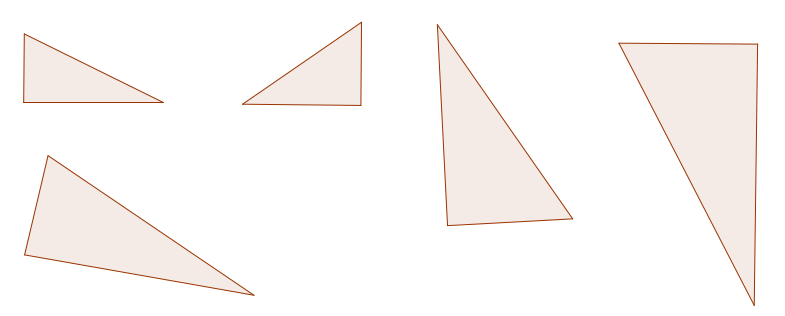
\includegraphics[width=0.7\linewidth]{5x5-aires-et-perimetres/ex2.pdf}
  \end{figure}
  
   \begin{figure}[H]
    \centering
    \includegraphics[width=0.7\linewidth]{5x5-aires-et-perimetres/ex3.pdf}
  \end{figure}
  
  \begin{figure}[H]
    \centering
    \includegraphics[width=0.7\linewidth]{5x5-aires-et-perimetres/ex4.pdf}
  \end{figure}
  
\end{minipage}
 \begin{minipage}[t]{0.7\textwidth}
   \Pointilles[40]
\end{minipage}

\newpage
\Pointilles[53]

\end{document}